% !TEX TS-program = pdflatex
% !TEX encoding = UTF-8 Unicode

% This is a simple template for a LaTeX document using the "article" class.
% See "book", "report", "letter" for other types of document.

\documentclass[11pt]{book} % use larger type; default would be 10pt

\usepackage[utf8]{inputenc} % set input encoding (not needed with XeLaTeX)

%%% Examples of Article customizations
% These packages are optional, depending whether you want the features they provide.
% See the LaTeX Companion or other references for full information.

%%% PAGE DIMENSIONS
\usepackage{geometry} % to change the page dimensions
\geometry{a4paper} % or letterpaper (US) or a5paper or....
% \geometry{margin=2in} % for example, change the margins to 2 inches all round
% \geometry{landscape} % set up the page for landscape
%   read geometry.pdf for detailed page layout information

\usepackage{graphicx} % support the \includegraphics command and options

% \usepackage[parfill]{parskip} % Activate to begin paragraphs with an empty line rather than an indent

%%% PACKAGES
\usepackage{booktabs} % for much better looking tables
\usepackage{array} % for better arrays (eg matrices) in maths
\usepackage{paralist} % very flexible & customisable lists (eg. enumerate/itemize, etc.)
\usepackage{verbatim} % adds environment for commenting out blocks of text & for better verbatim
\usepackage{subfig} % make it possible to include more than one captioned figure/table in a single float
% These packages are all incorporated in the memoir class to one degree or another...

%%% HEADERS & FOOTERS
\usepackage{fancyhdr} % This should be set AFTER setting up the page geometry
\pagestyle{fancy} % options: empty , plain , fancy
\renewcommand{\headrulewidth}{0pt} % customise the layout...
\lhead{}\chead{}\rhead{}
\lfoot{}\cfoot{\thepage}\rfoot{}

%%% SECTION TITLE APPEARANCE
\usepackage{sectsty}
\allsectionsfont{\sffamily\mdseries\upshape} % (See the fntguide.pdf for font help)
% (This matches ConTeXt defaults)

%%% ToC (table of contents) APPEARANCE
\usepackage[nottoc,notlof,notlot]{tocbibind} % Put the bibliography in the ToC
\usepackage[titles,subfigure]{tocloft} % Alter the style of the Table of Contents
\renewcommand{\cftsecfont}{\rmfamily\mdseries\upshape}
\renewcommand{\cftsecpagefont}{\rmfamily\mdseries\upshape} % No bold!

%%% END Article customizations

%%% The "real" document content comes below...
\begin{document}
\title{QSudoku}
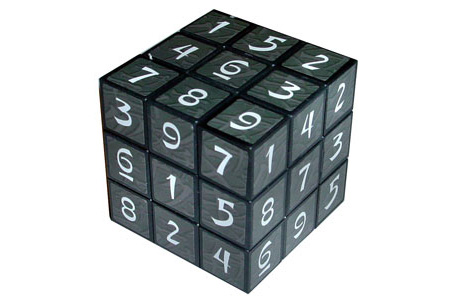
\includegraphics{sudo.jpg}
\author{Ramón Carrillo, Juan Mite,  Esteban Muñoz}
%\date{} % Activate to display a given date or no date (if empty),
         % otherwise the current date is printed 

\maketitle
\title{Índice}
\section{Introducción}
Es una aplicación realizada en lenguaje c++, utilizando el IDE Qt Creator, es una adaptación de famoso Sudoku, un pasatiempo que se publicó por primera vez a finales de la década de 1970 y se popularizó en Japón en 1986, dándose a conocer en el ámbito internacional en 2005 cuando numerosos periódicos empezaron a publicarlo en su sección de pasatiempos. 
\subsection{Descripción}
	El objetivo del sudoku es rellenar una cuadrícula de 9 x 9 celdas (81 casillas) dividida en subcuadrículas de 3 x 3 (también llamadas "cajas" o "regiones") con las cifras del 1 al 9 partiendo de algunos números ya dispuestos en algunas de las celdas. Aunque se podrían usar colores, letras, figuras, se conviene en usar números para mayor claridad, lo que importa, es que sean nueve elementos diferenciados, que no se deben repetir en una misma fila, columna o subcuadrícula. Un sudoku está bien planteado si la solución es única. La solución de un sudoku siempre es un cuadrado latino, aunque el recíproco en general no es cierto ya que el sudoku establece la restricción añadida de que no se puede repetir un mismo número en una región. 
\section{Manual de usuario}
\subsection{Pasos de la aplicación}

	Al lanzar la aplicación se mostrará una pantalla de inicio la cual permitirá al jugador registrarse, escoger la dificultad de juego, ver las estadísticas de juegos pasados, desarrolladores e iniciar su juego con los requisitos que especificó al inicio.
\subsection{Pantalla inicial}
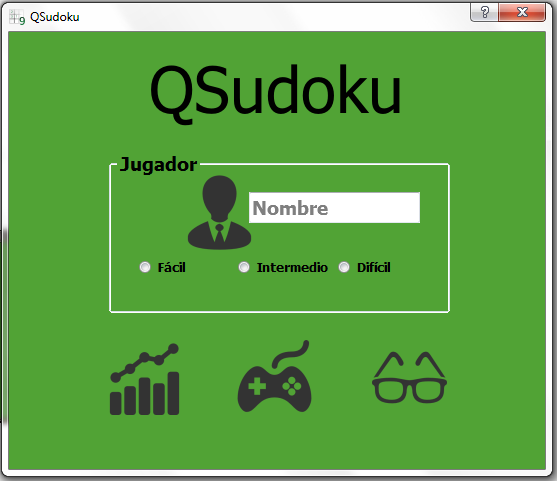
\includegraphics{inicio.png}
\subsection{Juego nuevo}
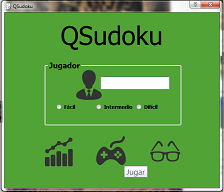
\includegraphics{Jugar.png}
\subsection{Estadísticas}
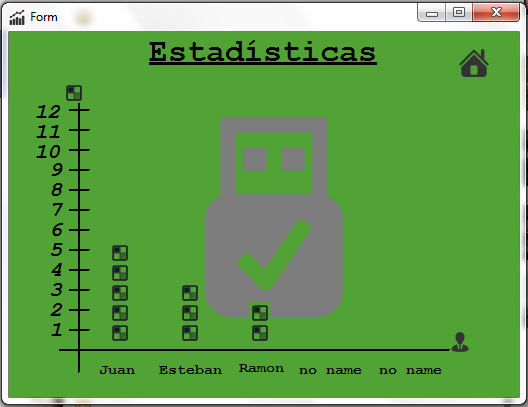
\includegraphics{estadist.png}
\subsection{Desarrolladores}
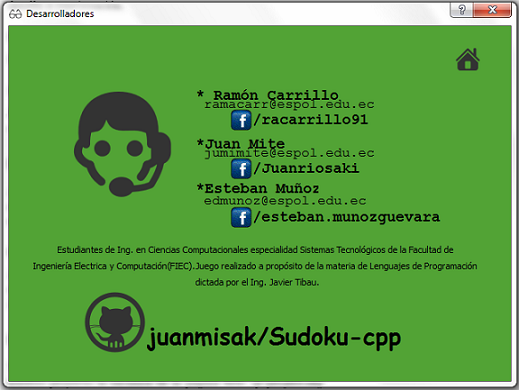
\includegraphics{pagdesa.png}
\section{Barra de menú}
\subsection{Sudoku /Juego Nuevo}
\subsection{Sudoku /Salir}
\section{Acerca de}
\subsection{Desarrolladores}
\section{Bibliografía}

\title{Desarrolladores}
\maketitle
		Juan Mite 
		Daniel Muñoz
		Ramón Carrillo
	Estudiantes de la Escuela Superior Politécnica del Litoral a propósito de la materia de Lenguajes de programación dictada por el Ing. Javier Tibau profesor de la Facultad de Ingeniería Eléctrica y Computación.  

\end{document}

